%%%%%%%%%%%%%%%%%%%%%%%%%%%%%%%%%%%%%%%%%%%%%%%%%%%%%%%%%%%%%%%%%
\chapter{Configuración del Entorno}
\label{ch:environment-setup}
%%%%%%%%%%%%%%%%%%%%%%%%%%%%%%%%%%%%%%%%%%%%%%%%%%%%%%%%%%%%%%%%%

Este capítulo recorre la instalación de todo el software requerido
para el proyecto \ProjectName{}. Complete las secciones
obligatorias en orden antes de la primera sesión. Las secciones opcionales pueden
completarse en cualquier momento. Las instrucciones están escritas principalmente para
Windows, pero incluyen pasos equivalentes para macOS y Linux a lo largo del texto.

\vs
\noindent
La familiaridad con la línea de comandos y con las rutas de archivos es útil, pero
no es requerida aquí. Estos conceptos se cubren completamente en
el Capítulo~\ref{ch:cli-scripting}, que puede leer después de completar
este capítulo.
\vs

%================================================================
\section{Obligatorio: Instalar Python}\label{sec:python}
%================================================================

Instale cualquier versión reciente de Python desde \href{https://www.python.org/downloads/}{https://www.python.org/downloads/}. Vaya a sus descargas y haga doble clic en el archivo de instalación para iniciar la instalación. Por defecto, el instalador de Python para Windows coloca sus ejecutables en el directorio AppData del usuario, de modo que no requiere permisos administrativos. Esto funciona para la mayoría de los escenarios. Si usted es el único usuario en el sistema, podría preferir colocar Python en un directorio de nivel superior (por ejemplo, \texttt{C:\textbackslash Python} o \texttt{/usr/local/bin}) para tener una ruta más corta a los binarios (a veces necesitará eso). Dependiendo de sus preferencias, seleccione «\textit{Install Now}» o «\textit{Customized installation}» (mi preferencia). Asegúrese de seleccionar «\textit{Add python.exe to path}»; esto le ahorrará algunos dolores de cabeza más adelante.

\begin{figure}[htbp]
	\centering
	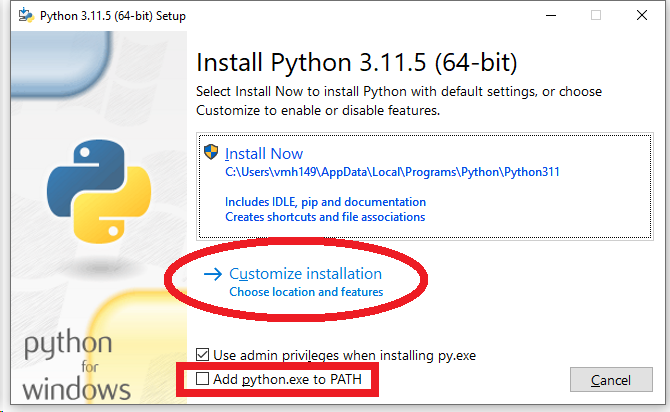
\includegraphics[width=0.65\textwidth]{../images/envsetup-3-1.png}
	\caption{Instalador de Python mostrando la casilla «Add python.exe to PATH» en la parte inferior.}
	\label{fig:envsetup-3-1}
\end{figure}

En la ventana «Optional Features» seleccione todas las características.

\begin{figure}[htbp]
	\centering
	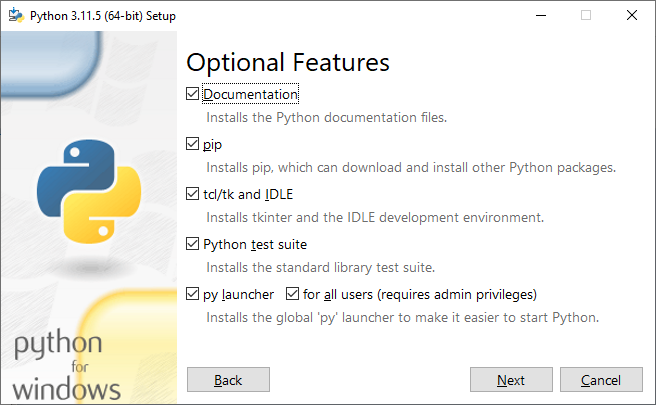
\includegraphics[width=0.65\textwidth]{../images/envsetup-4-1.png}
	\caption{Pantalla de características opcionales de Python: seleccione todas las características.}
	\label{fig:envsetup-4-1}
\end{figure}

Seleccione «\textit{Install Python X.XX for all users}» si puede y lo desea. Esto requiere privilegios administrativos. Seleccione la carpeta de su elección para la ubicación de instalación.

\begin{figure}[htbp]
	\centering
	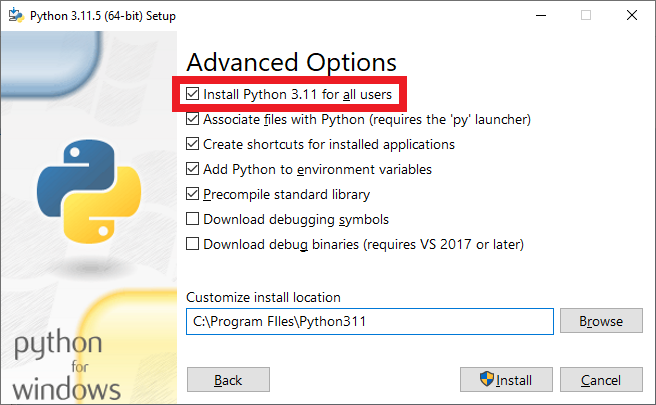
\includegraphics[width=0.65\textwidth]{../images/envsetup-4-2.png}
	\caption{Pantalla de opciones avanzadas de Python mostrando «Install for all users» seleccionado.}
	\label{fig:envsetup-4-2}
\end{figure}

Para PC: Si no agregó \texttt{python.exe} al PATH durante la instalación, espere hasta que la instalación se complete. Luego abra el Explorador de archivos y haga clic derecho sobre «Este equipo». Seleccione «Propiedades» del menú contextual. En la ventana del Sistema que se abre, haga clic en «Configuración avanzada del sistema» en la barra lateral izquierda. En la nueva ventana, asegúrese de que la pestaña «Opciones avanzadas» esté seleccionada y haga clic en el botón «Variables de entorno» cerca de la parte inferior. Bajo la sección «Variables del sistema», busque y haga doble clic en la variable llamada «Path». Esto abrirá una ventana donde podrá agregar la ruta al ejecutable de Python manualmente.

\vs

Para Mac: Si no se aseguró de que Python fuera agregado al PATH de su sistema durante la instalación, puede hacerlo manualmente usando los siguientes pasos en una Mac. Después de que la instalación esté completa, abra la aplicación Terminal. Ingrese el comando \texttt{which python3} o \texttt{which python} para encontrar la ruta al binario de Python instalado. Copie esa ruta. Luego abra su archivo de configuración del intérprete de comandos en un editor de texto. Este será típicamente \texttt{\~{}/.zshrc} si está usando el shell Zsh (predeterminado en versiones más recientes de macOS) o \texttt{\~{}/.bash\_profile} si está usando Bash. Agregue la línea \texttt{export PATH="/path/to/python:\$PATH"}, reemplazando \texttt{/path/to/python} con la ruta que copió. Guarde el archivo y cierre el editor. En la Terminal, ejecute \texttt{source \~{}/.zshrc} o \texttt{source \~{}/.bash\_profile} dependiendo del archivo que editó, para que el nuevo PATH se cargue en su entorno.

%================================================================
\section{Opcional (pero \underline{muy} recomendado): Instalar una distribución de \LaTeX{}}\label{sec:latex-install}
%================================================================

\LaTeX{} es un sistema de composición tipográfica de alta calidad diseñado para la creación de
documentos técnicos y científicos. En lugar de formatear el texto visualmente,
los autores escriben archivos fuente en texto plano usando un lenguaje de marcado que describe
la estructura y el significado del contenido (como secciones, ecuaciones,
y referencias). Estos archivos fuente se compilan luego en documentos
profesionalmente formateados (típicamente PDFs). \LaTeX{} destaca en la composición de
ecuaciones, la gestión de referencias cruzadas, y la producción de salida consistente y
de calidad de publicación, lo que lo convierte en la herramienta estándar para muchos campos
en ciencia, ingeniería y matemáticas.

\begin{infobox}
	\LaTeX{} es particularmente adecuado para la interacción con los Modelos Grandes de Lenguaje
\end{infobox}


\LaTeX{} es particularmente adecuado para la interacción con los Modelos Grandes de Lenguaje
(LLMs) porque es un lenguaje de marcado puramente textual y declarativo que se asemeja
estrechamente al código fuente estructurado. A diferencia de los formatos de documento binarios (por ejemplo, Word o PDF),
un documento de \LaTeX{} expone su estructura lógica completa---secciones, ecuaciones,
entornos y referencias---en texto plano. Esto lo hace directamente
interpretable, editable y generable por los LLMs, que están fundamentalmente
entrenados y optimizados para texto y código. Como resultado, los LLMs pueden asistir
de manera fiable en tareas como la redacción de contenido matemático, la refactorización de estructura,
la verificación de notación e incluso la depuración de problemas de compilación. En este sentido,
\LaTeX{} sirve como una interfaz natural entre el razonamiento matemático humano
y la generación asistida por máquina, permitiendo flujos de trabajo de documentos
precisos, reproducibles y automatizables.

\LaTeX{} es requerido si planea compilar documentos \texttt{.tex}
localmente. Los documentos del programa se mantienen como archivos fuente \LaTeX{}
en el repositorio. Para la autoría y compilación de sus propios
documentos, instale la distribución para su plataforma.


\begin{table}[htbp]
\centering
\caption{Distribuciones de \LaTeX{} recomendadas por plataforma}
\label{tab:latex-distros}
\begin{tabular}{llp{7.5cm}}
\toprule
\textbf{Plataforma} & \textbf{Distribución} & \textbf{Descarga} \\
\midrule
Windows & MiKTeX & \url{https://miktex.org} \\
macOS & MacTeX & \url{https://www.tug.org/mactex/} \\
Linux (Ubuntu/Debian) & TeX Live & \texttt{sudo apt install texlive-latex-extra texlive-fonts-recommended latexmk} \\
\bottomrule
\end{tabular}
\end{table}

Verifique la instalación en cualquier plataforma con:

\begin{verbatim}
pdflatex --version
\end{verbatim}

\vs
\noindent
El uso de \LaTeX{} para la preparación de documentos, incluyendo una hoja
de referencia de notación matemática, se cubre en el Capítulo~\ref{ch:latex}.
\vs

%================================================================
\section{Obligatorio: Instalar Visual Studio Code (VSC)}\label{sec:vsc}
%================================================================

\textbf{Si usted es nuevo en Python, instale \href{https://code.visualstudio.com}{Visual Studio Code} (VSC)}: Hay muchas opciones para escribir código Python, y usted podría tener una favorita. Debo elegir una para impartir la instrucción, y la experiencia me ha mostrado que VSC ofrece la menor cantidad de fricción.

\vs

En VSC, hay dos opciones principales: «\textit{User Installer}» y «\textit{System Installer}». Use el User Installer si desea instalar solo para el usuario actual. Para todos los usuarios, use el System Installer; yo prefiero esta opción porque instala VSC en \texttt{C:\textbackslash Program Files\textbackslash Microsoft VS Code}.

\vs

Visual Studio Code está disponible para Windows, macOS y Linux; una alternativa idéntica de código abierto llamada VSCodium está disponible en \url{https://vscodium.com}.

%================================================================
\section{Obligatorio: Extensiones de Visual Studio Code}\label{sec:extensions}
%================================================================

Seleccione el ícono de Extensiones a la izquierda e instale las siguientes bibliotecas de Visual Studio Code.

\begin{enumerate}
	\item \textbf{Obligatorio}: Extensión de Python para Visual Studio Code.

	\item \textbf{Opcional}: Instale también Jupyter (esto también instala Pylance, Jupyter Keymap, Jupyter Notebook Renderers, Jupyter SlideShow). Preste atención al editor de la extensión; use las de Microsoft.

	\begin{figure}[htbp]
		\centering
		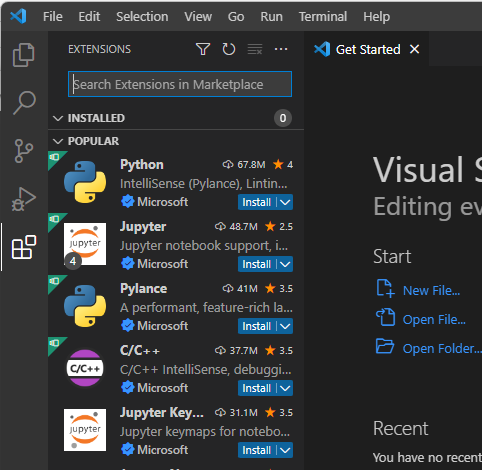
\includegraphics[width=0.7\textwidth]{../images/envsetup-5-1.png}
		\caption{Mercado de Extensiones de VS Code mostrando las extensiones de Python y Jupyter de Microsoft.}
		\label{fig:envsetup-5-1}
	\end{figure}

	\item \textbf{Opcional}: Instale C/C++ para Visual Studio Code, C/C++ Themes y C/C++ Extension Pack.

	\item \textbf{Opcional}: Instale la extensión «\textbf{LaTeX Workshop}» de James Yu. Esta extensión proporciona resaltado de sintaxis, vista previa en vivo y compilación con un clic. Su uso se describe en la Sección~\ref{sec:latex-workshop}.

	\begin{figure}[htbp]
		\centering
		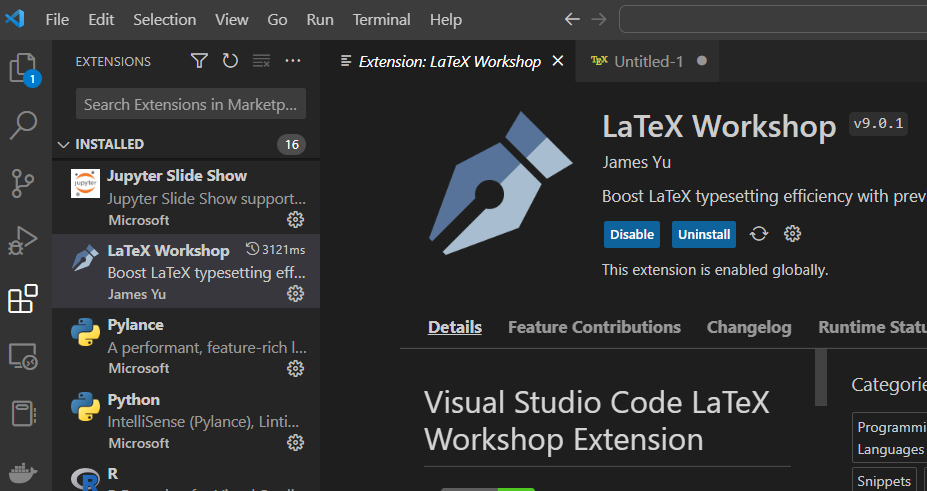
\includegraphics[width=0.7\textwidth]{../images/envsetup-6-1.png}
		\caption{Página de la extensión LaTeX Workshop en VS Code.}
		\label{fig:envsetup-6-1}
	\end{figure}
\end{enumerate}

%================================================================
\section{Opcional: Windows Terminal}\label{sec:terminal}
%================================================================

Para usuarios de Windows, instale \href{https://apps.microsoft.com/detail/windows-terminal}{Windows Terminal}. Esta aplicación de Microsoft le permite utilizar una ventana de múltiples documentos con pestañas para diferentes consolas de comandos como PowerShell, Ubuntu, DOS, Git, etc. Necesitará esto si desea completar los pasos relacionados con Linux en la siguiente sección de este documento.

%================================================================
\section{Obligatorio: Instalar Git}\label{sec:git}
%================================================================

Instale \href{https://gitforwindows.org}{Git for Windows}. Para Mac, instale \href{https://git-scm.com/download/mac}{Git for Mac}. Linux también tiene una versión disponible. En la segunda pantalla, seleccione Visual Studio Code como su editor de Git. Use todas las demás opciones predeterminadas.

\begin{figure}[htbp]
	\centering
	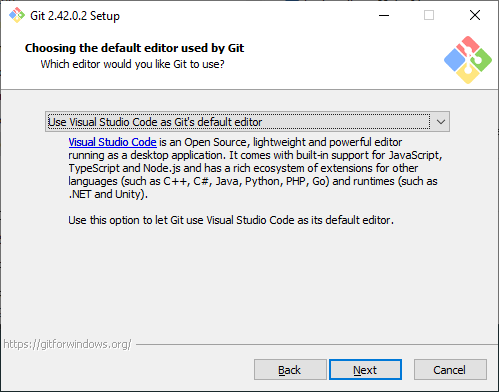
\includegraphics[width=0.6\textwidth]{../images/envsetup-2-1.png}
	\caption{Pantalla de configuración de Git mostrando Visual Studio Code como el editor predeterminado.}
	\label{fig:envsetup-2-1}
\end{figure}

%================================================================
\section{Obligatorio: Abrir Git Bash (o cualquier terminal)}\label{sec:gitbash}
%================================================================

La línea de comandos le permite controlar su computadora escribiendo instrucciones, proporcionando acceso preciso a los archivos y características del sistema. Por ejemplo, al escribir \texttt{ls} en un sistema tipo Unix como Linux o macOS se lista los archivos y directorios en la ubicación actual, por ejemplo \texttt{ls /home/user/Documents} para mostrar el contenido de la carpeta Documents. En Windows, el comando \texttt{dir} cumple la misma función, de modo que \texttt{dir C:\textbackslash Users\textbackslash Alice\textbackslash Desktop} muestra lo que hay en el Escritorio. Para moverse entre directorios, se usa el comando \texttt{cd}; \texttt{cd Downloads} cambia el directorio de trabajo a Downloads, mientras que \texttt{cd ..} sube un nivel. Estos comandos permiten la navegación e inspección eficiente del sistema de archivos a través de la terminal.

\vs

Ahora que Git está instalado, clone el repositorio de \ProjectName{}.
Abra Git Bash (Windows) o una terminal (macOS/Linux),
navegue a la carpeta donde desea almacenar el proyecto, y ejecute:

{\ttfamily \noindent
git clone \ProjectGit.git
}

Esto crea una carpeta llamada \texttt{\ProjectFolder} que contiene todos
los materiales del taller. Solo necesita hacer esto una vez. Para actualizar su
copia local más adelante, navegue dentro de la carpeta y ejecute \texttt{git pull}.

%================================================================
\section{Obligatorio: Abrir el proyecto \ProjectName{} en Visual Studio Code}\label{sec:vscstart}
%================================================================

Para abrir el proyecto \ProjectName{} en VSC, abra una terminal, navegue dentro de la
carpeta \texttt{\ProjectFolder} que clonó en la sección anterior,
y ejecute:

{\ttfamily \noindent
cd \ProjectFolder \\
code .
}

El punto después de \texttt{code} instruye a VSC para usar la carpeta actual
como la carpeta de trabajo. Todos los archivos del taller serán visibles en el
explorador de archivos de VSC.

%================================================================
\section{Obligatorio: Instalar bibliotecas de Python}\label{sec:libraries}
%================================================================

Las bibliotecas de Python para el desafío de datos se instalan dentro de un entorno
virtual. Complete el Capítulo~\ref{ch:python-environments} para configurar
su entorno, luego instale las bibliotecas requeridas como se describe allí.

%================================================================
\section{Opcional: Jupyter Notebook}\label{sec:jupyter}
%================================================================

\textbf{Opcional}: Ahora, cree un Jupyter Notebook.

\begin{enumerate}
	\item Abundante información relevante sobre Jupyter en VSC está disponible en \href{https://code.visualstudio.com/docs/datascience/jupyter-notebooks}{https://code.visualstudio.com/docs/datascience/jupyter-notebooks}

	\item Active el entorno que desea usar (véase el Capítulo~\ref{ch:python-environments}).

	\item Necesita adjuntar el kernel de su entorno virtual. Por ejemplo, si tengo un entorno virtual llamado venn:

	\begin{verbatim}
	python -m ipykernel install --user --name=venn
	\end{verbatim}

	\item Abra VS Code en la carpeta de su proyecto (véase la Sección~\ref{sec:vscstart}).

	\item En VSC, ejecute el comando \texttt{Create:New Jupyter Notebook} desde la Paleta de Comandos (Ctrl+Shift+P) o creando un nuevo archivo .ipynb en su espacio de trabajo.

	\item Podría recibir una alerta de seguridad respecto al firewall. Permita el acceso.

	\begin{figure}[htbp]
		\centering
		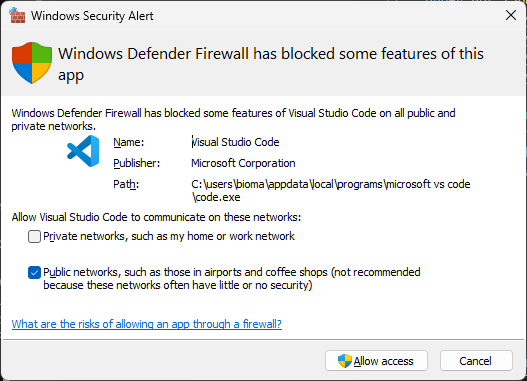
\includegraphics[width=0.6\textwidth]{../images/envsetup-14-1.png}
		\caption{Alerta del Firewall de Windows Defender: permita el acceso para Visual Studio Code.}
		\label{fig:envsetup-14-1}
	\end{figure}

	\item Después de ingresar un comando, podría ver el siguiente mensaje:

	\begin{figure}[htbp]
		\centering
		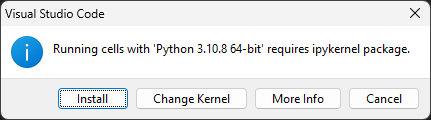
\includegraphics[width=0.55\textwidth]{../images/envsetup-14-2.png}
		\caption{Indicación de VS Code para instalar el paquete ipykernel: haga clic en Instalar.}
		\label{fig:envsetup-14-2}
	\end{figure}

	Instálelo.
\end{enumerate}

%================================================================
\section{Opcional: Comandos de Python en la Terminal}\label{sec:pythonterminal}
%================================================================

Finalmente, usted puede simplemente ingresar comandos de Python en la Terminal. Abra un símbolo del sistema y escriba el siguiente comando:

\begin{verbatim}
python
\end{verbatim}

Esto le permitirá ingresar comandos de Python, por ejemplo \texttt{1+1}

%================================================================
\section{Solución de problemas}\label{sec:troubleshoot}
%================================================================

Los siguientes errores han sido reportados por participantes anteriores.
Si encuentra un problema diferente, consulte el rastreador de problemas del repositorio
de \ProjectName{} en \url{\ProjectGit/issues}.

\vs

Según lo reportado por Lorena Roa de La Cruz, podría ver un error al intentar activar un entorno virtual. Esto se debe a la configuración de permisos. Si esto sucede, ejecute el comando:

\begin{verbatim}
Set-ExecutionPolicy -ExecutionPolicy RemoteSigned -Scope CurrentUser
\end{verbatim}

Después de eso, ejecute el script \texttt{activate}.

\begin{figure}[htbp]
	\centering
	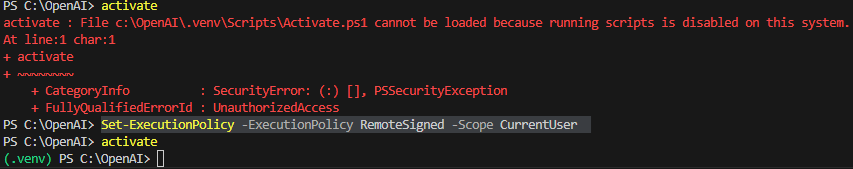
\includegraphics[width=0.85\textwidth]{../images/envsetup-12-1.png}
	\caption{Error de política de ejecución de PowerShell y solución: ejecución de \texttt{Set-ExecutionPolicy} seguido de \texttt{activate}.}
	\label{fig:envsetup-12-1}
\end{figure}

%================================================================
\section{Opcional: Compiladores de C/C++}\label{sec:compilers}
%================================================================

Si desea programar en C o C++, tiene varias opciones, incluyendo \href{https://gcc.gnu.org}{GCC, the GNU Compiler Collection}, pero requiere cierto esfuerzo instalar los prerrequisitos. De Microsoft existe \href{https://visualstudio.microsoft.com/vs/community/}{Visual Studio Community Edition} (VSCE), que encapsula la complejidad de instalar múltiples compiladores (incluyendo el SDK del marco de trabajo .NET). Le recomiendo que instale VSCE con todas las «Workloads» en «Web \& Cloud» y «Desktop \& Mobile» (excepto Python).

%================================================================
\section{Opcional: Instalación de PostgreSQL en Linux}
%================================================================
Muchas distribuciones de Linux incluyen versiones antiguas de PostgreSQL en sus
repositorios predeterminados. Para instalar la última versión estable, se recomienda
utilizar el repositorio oficial de paquetes de PostgreSQL mantenido por el
PostgreSQL Global Development Group.

El siguiente procedimiento instala la versión estable más reciente en
sistemas Ubuntu o Debian.

%----------------------------------------------------------------
\subsection{Instalar las utilidades requeridas}
%----------------------------------------------------------------
Primero instale las utilidades requeridas para recuperar y verificar paquetes.

\begin{lstlisting}[basicstyle=\footnotesize\ttfamily]
sudo apt update
sudo apt install curl ca-certificates
\end{lstlisting}

%----------------------------------------------------------------
\subsection{Agregar el repositorio de PostgreSQL}
%----------------------------------------------------------------
Agregue el repositorio oficial de PostgreSQL a las fuentes de paquetes del sistema.

\begin{lstlisting}[basicstyle=\footnotesize\ttfamily]
sudo sh -c 'echo "deb http://apt.postgresql.org/pub/repos/apt \
$(lsb_release -cs)-pgdg main" \
> /etc/apt/sources.list.d/pgdg.list'
\end{lstlisting}

%----------------------------------------------------------------
\subsection{Importar la clave de firma del repositorio}
%----------------------------------------------------------------
Importe la clave de firma del repositorio de PostgreSQL.

\begin{lstlisting}[basicstyle=\footnotesize\ttfamily]
curl -fsSL https://www.postgresql.org/media/keys/ACCC4CF8.asc \
| sudo gpg --dearmor -o /usr/share/keyrings/postgresql.gpg
\end{lstlisting}

Actualice la configuración del repositorio para referenciar la clave.

\begin{lstlisting}[basicstyle=\footnotesize\ttfamily]
sudo nano /etc/apt/sources.list.d/pgdg.list
\end{lstlisting}

Modifique la línea para que se lea en una sola línea (el carácter \textbackslash{}  significa retorno de línea; está aquí solo para indicar que todo es una sola línea; elimínelo y una las siguientes tres líneas de texto en una sola línea):

\begin{lstlisting}[basicstyle=\footnotesize\ttfamily]
deb [signed-by=/usr/share/keyrings/postgresql.gpg] \
http://apt.postgresql.org/pub/repos/apt \
$(lsb_release -cs)-pgdg main
\end{lstlisting}

%----------------------------------------------------------------
\subsection{Instalar PostgreSQL}
%----------------------------------------------------------------
Actualice el índice de paquetes e instale la última versión de PostgreSQL.

\begin{lstlisting}[basicstyle=\footnotesize\ttfamily]
sudo apt update
sudo apt install postgresql-16
\end{lstlisting}

%----------------------------------------------------------------
\subsection{Verificar la instalación}
%----------------------------------------------------------------
Confirme que PostgreSQL se instaló correctamente.

\begin{lstlisting}[basicstyle=\footnotesize\ttfamily]
psql --version
\end{lstlisting}

La salida debería indicar la versión instalada de PostgreSQL.

%----------------------------------------------------------------
\subsection{Iniciar el servidor de base de datos}
%----------------------------------------------------------------
Si el servicio aún no está en ejecución, inicie el clúster de PostgreSQL.

\begin{lstlisting}[basicstyle=\footnotesize\ttfamily]
sudo systemctl start postgresql
\end{lstlisting}

Verifique el estado del servidor:

\begin{lstlisting}[basicstyle=\footnotesize\ttfamily]
sudo systemctl status postgresql
\end{lstlisting}

%----------------------------------------------------------------
\subsection{Acceder al intérprete de comandos de PostgreSQL}
%----------------------------------------------------------------
Para abrir la terminal interactiva de PostgreSQL:

\begin{lstlisting}[basicstyle=\footnotesize\ttfamily]
sudo -u postgres psql
\end{lstlisting}

Salga del intérprete de comandos usando:

\begin{lstlisting}[basicstyle=\footnotesize\ttfamily]
\q
\end{lstlisting}
